
\subsection{中性子輸送方程式}
ここからは、定義した中性子束・中性子流から厳密に正しい中性子の輸送に関する
方程式、「\emph{中性子輸送方程式}」を導出する。

\subsubsection{中性子輸送方程式の設計図}
まず、厳密に正しい中性子輸送を記述するには何が必要かを考える、
すなわち、方程式の設計図を作成していくこととする。
出発点として、中性子輸送方程式を
\begin{itemize}[label={}]
  \item ある時刻$t$に
  \item 位置$\mathbf{r}$まわりの体積$dV$内に存在し、
  \item エネルギーが$E$まわりの幅$dE$内にあり、
  \item 方向$\SpcAng$まわりの$d\SpcAng$に向かって飛行する
  \item 中性子数の期待値
\end{itemize}
すなわち角度中性子密度$n(\rEOt)$の時間変化に着目した方程式と捉えよう。
角度中性子密度の時間変化に影響を与えるものとして、次の項目がある。
\begin{align}
  \frac{\partial n(\rEOt)}{\partial t} &= \text{角度中性子密度の時間変化} \notag \\
   &= \text{生成率} - \text{消滅率} \notag \\
   &= \text{(空間的な流入以外の)生成率} - (\text{漏洩率} + \text{吸収率} + \text{散乱で失われる率})
\end{align}

\subsubsection{生成率}
角度中性子密度を増加させる要因としては次のものが考えられる。
\vskip.5\baselineskip
\subparagraph{中性子源による生成}
位置$\mathbf{r}$まわりの体積$dV$内に中性子源がある場合、
中性子数は増加する。線源によって$n(\rEOt)$にカウントされる
中性子を放出する数を$s(\rEOt)$とする。
これを\emph{中性子線源項}と呼ぶ。
\begin{itembox}[l]{中性子線源項}
  \begin{equation}
    \text{中性子源による生成率} = s(\rEOt) \label{source}
  \end{equation}
\end{itembox}

\newpage
\subparagraph{散乱による生成}
\newcommand{\EOtoEO}{E' \rightarrow E, \SpcAng' \rightarrow \SpcAng}
\begin{itemize}[label={}]
  \item ある時刻$t$に
  \item 位置$\mathbf{r}$まわりの体積$dV$内に存在し、
  \item 他のエネルギー$E'$周りの幅$dE'$内で
  \item 方向$\SpcAng'$まわりの$d\SpcAng'$の方向に飛行する中性子
\end{itemize}
が、散乱によって$n(\rEOt)$にカウントされる中性子になる場合も生成として捉える。
$E'$からの散乱による生成率は
\begin{align}
  \text{$E'$、$\SpcAng'$からの散乱による生成率}
   = \Sigma_s (\mathbf{r}, \EOtoEO) v(E') n(\mathbf{r}, E', \SpcAng', t)
\end{align}
エネルギーと立体角について積分すれば、散乱による生成率を表現できる。
これを\emph{散乱流入項}と呼ぶ。
\begin{itembox}[l]{散乱流入項}
  \begin{equation}
    \text{散乱による生成率}
     = \int_{4 \pi} \int_{0}^{\infty} \Sigma_s (\mathbf{r}, \EOtoEO) v(E') n(\mathbf{r}, E', \SpcAng', t) \ dE' d\SpcAng' \label{inscattering}
  \end{equation}
\end{itembox}
$\Sigma_s (\mathbf{r}, \EOtoEO)$はエネルギー依存、立体角依存の
散乱断面積であり、2重微分断面積と呼ぶ。

\subsubsection{漏洩率}
漏洩率では\emph{空間的な流入・流出}を同時に取り扱う。
領域$V$を設定し、その表面$S$の微小面積$\Delta S$を考え、その面に対する外向きの
単位法線ベクトル$\nhat$とおく。まず、$\Delta S$を
単位時間あたりに通過する$\SpcAng$方向の速さ$v$の中性子数について数式で表現する。
これは、微小面積$\Delta S$を長さ$v$だけ$\SpcAng$方向に動かした際にできる
微小体積$\Delta V$内に存在する中性子数に等しくなるはずである。よって、
正味の流量は以下で表せる。
\begin{align}
  \Delta V = v \nhat \cdot \SpcAng \Delta S \ \text{なので、}\notag \\
  n(\rEOt) v(E) \nhat \cdot \SpcAng \Delta S
\end{align}
領域$V$全体で考えるなら表面$S$で積分すればよく、
\begin{align}
  \text{領域$V$からの漏洩率} &= \int_{S} \nhat \cdot \SpcAng v(E) n(\rEOt) \ dS \notag \\
  &= \int_{S} \nhat \cdot \SpcAng \psi(\rEOt) \ dS \quad \text{ガウスの発散定理から}\\
  &= \int_{V} \mathrm{div} \ \SpcAng \psi(\rEOt) \ dV \label{V-lossterm} 
\end{align}
 $\nabla = \left( \frac{\partial}{\partial x},
 \frac{\partial}{\partial y}, \frac{\partial}{\partial z}\right)$
を用いれば、
\begin{align}
  \int_{V} \mathrm{div} \ \SpcAng \psi(\rEOt) \ dV &= \int_{V} \nabla \SpcAng \psi(\rEOt) \ dV \notag\\
  \text{$\SpcAng$が空間$\mathbf{r}=(x,y,z)$に依存しないので} \quad &= \int_{V} \SpcAng \cdot \nabla \psi(\rEOt) \ dV
\end{align}
式~\eqref{V-lossterm}を体積$V$で割り、$V \rightarrow 0$と
すると、単位体積あたりの漏洩率となる
\footnote{$\psi$がスカラー量なので$\nabla \psi$はベクトルを与える}。
\begin{itembox}[l]{漏洩率}
  \begin{equation}
    \text{漏洩率}
     = \SpcAng \cdot \nabla \psi(\rEOt) \label{lossterm-flux}
  \end{equation}
  あるいは、角度中性子流を使って
  \begin{equation}
    \nabla \cdot \mathbf{j}(\rEOt)  \label{lossterm-crnt}
  \end{equation}
\end{itembox}

\subsubsection{吸収率}
吸収される量は巨視的吸収反応断面積を$\Sigma_a$とおいて次で表される。
\begin{itembox}[l]{吸収率}
  \begin{equation}
    \text{吸収率}
     = \Sigma_a v(E) n(\rEOt) \label{absorptionterm}
  \end{equation}
\end{itembox}

\subsubsection{散乱で失われる率}
散乱で失われる量は巨視的散乱断面積を$\Sigma_s$とおいて次で表される。
\begin{itembox}[l]{散乱で失われる率}
  \begin{equation}
    \text{散乱で失われる率}
     = \Sigma_s v(E) n(\rEOt) \label{scatteringterm}
  \end{equation}
\end{itembox}

\subsubsection{微積分型中性子輸送方程式}
ここまでに表現した項を組み合わせて「微積分型」の中性子輸送方程式を
組み立てる。

\begin{align}
  \frac{\partial n(\rEOt)}{\partial t}
   &= s(\rEOt) \notag \\
   &+ \int_{4 \pi} \int_{0}^{\infty} \Sigma_s (\mathbf{r}, \EOtoEO) v(E') n(\mathbf{r}, E', \SpcAng', t) \ dE' d\SpcAng' \notag \\
   &- \left(
  \begin{aligned}
   &\quad \SpcAng \cdot \nabla \psi(\rEOt) \\
   &+ \Sigma_a v(E) n(\rEOt) \\
   &+ \Sigma_s v(E) n(\rEOt)
  \end{aligned}
   \right) \label{transport-pre}
\end{align}

式~\eqref{transport-pre}について、巨視的断面積について、
全断面積$\Sigma_t$は$\Sigma_t = \Sigma_a + \Sigma_s$、
式の左辺は
$\frac{\partial n(\rEOt)}{\partial t} = \frac{1}{v(E)} \frac{\partial \psi(\rEOt)}{\partial t}$
である。そこで、式に出てくる角度中性子密度を角度中性子束に置き換えて、
消滅側の断面積の項をまとめると次の形にできる。
\vskip.5\baselineskip
\begin{itembox}[l]{微積分型中性子輸送方程式}
  \begin{align}
    \frac{1}{v(E)} \frac{\partial \psi(\rEOt)}{\partial t}
     &= s(\rEOt) \notag \\
     &+ \int_{4 \pi} \int_{0}^{\infty} \Sigma_s (\mathbf{r}, \EOtoEO) \psi(\mathbf{r}, E', \SpcAng', t) \ dE' d\SpcAng' \notag \\
     &- \SpcAng \cdot \nabla \psi(\rEOt) - \Sigma_t \psi(\rEOt) \label{transport}
  \end{align}
\end{itembox}
\vskip.5\baselineskip
これが微積分型の中性子輸送方程式である。

\subsubsection{臨界状態の中性子輸送方程式}
\newcommand{\rEO}{\mathbf{r}, E, \SpcAng} % 文字の()内変数
臨界状態の原子炉では角度中性子束は定常状態となり、時間変化は$0$となる。
また、中性子源は原子炉自身の核分裂となる。
中性子源が核分裂である場合の線源項は、
巨視的核分裂断面積を$\Sigma_f$、
核分裂あたりの平均中性子発生数を$\nu$
核分裂中性子のエネルギースペクトルを$\chi$とすれば、
核分裂中性子は等方的に放出されるので、
\begin{equation}
  s(\rEOt) = \frac{\chi(E)}{4 \pi} 
  \int_{4 \pi} \int_{0}^{\infty} \nu \Sigma_f(\mathbf{r}, E') \psi(\mathbf{r}, E', \SpcAng') \ dE' d\SpcAng'
\end{equation}

これを式~\eqref{transport}に代入すれば臨界状態の微積分型輸送方程式になる。

\begin{align}
  &\SpcAng \cdot \nabla \psi(\rEO) + \Sigma_t \psi(\rEO) \notag \\
  &= \int_{4 \pi} \int_{0}^{\infty} \Sigma_s (\mathbf{r}, \EOtoEO) \psi(\mathbf{r}, E', \SpcAng') \ dE' d\SpcAng' \notag \\
  &+ \frac{\chi(E)}{4 \pi} 
  \int_{4 \pi} \int_{0}^{\infty} \nu \Sigma_f(\mathbf{r}, E') \psi(\mathbf{r}, E', \SpcAng') \ dE' d\SpcAng'
\end{align}
式を書くのが煩雑になるので、生成項部分をまとめて文字で置いて
\begin{equation}
  \SpcAng \cdot \nabla \psi(\rEO) + \Sigma_t \psi(\rEO) = Q(\rEO) \label{transport-crit}
\end{equation}

\subsubsection{積分型中性子輸送方程式}
微積分型の輸送方程式を積分することで全く等価な積分型の式に変形できる。
数値的に解を求める場合、一般的には微分値よりも積分値の方が精度が良いため、
この輸送方程式が用いられる。炉心の燃料格子系(燃料集合体内等)の中性子束を
計算する場合は、積分型中性子輸送方程式を基にした「衝突確率法」がよく使われる。

微積分型中性子輸送方程式~\eqref{transport}について、
式~\eqref{transport-crit}のように生成項を$Q$にまとめる。
\begin{align}
  &Q(\rEOt) = \notag \\
  &\int_{4 \pi} \int_{0}^{\infty} 
   \Sigma_s (\mathbf{r}, \EOtoEO) \psi(\mathbf{r}, E', \SpcAng', t) \ dE' d\SpcAng'
   + s(\rEOt) \label{sourceQ}\\
  &\text{したがって、輸送方程式は}\notag \\
  &\left( 
    \frac{1}{v(E)}\frac{\partial}{\partial t} + \SpcAng \cdot \nabla + \Sigma_t(\mathbf{r},E)
   \right) \psi(\rEOt) = Q(\rEOt) \label{trans-Q}
\end{align}

ここで、「中性子の飛行経路に沿って少し巻き戻されたときの変化率」
を表す微分を考えてみる。Fig.~\ref{path-s}で図示したように、中性子の飛行方向$\SpcAng$の長さを
$s$としてこの長さだけ巻き戻された座標$\mathbf{r}'$と時刻$t'$を表現すると、
\begin{figure}[htbp]
  \begin{center}
  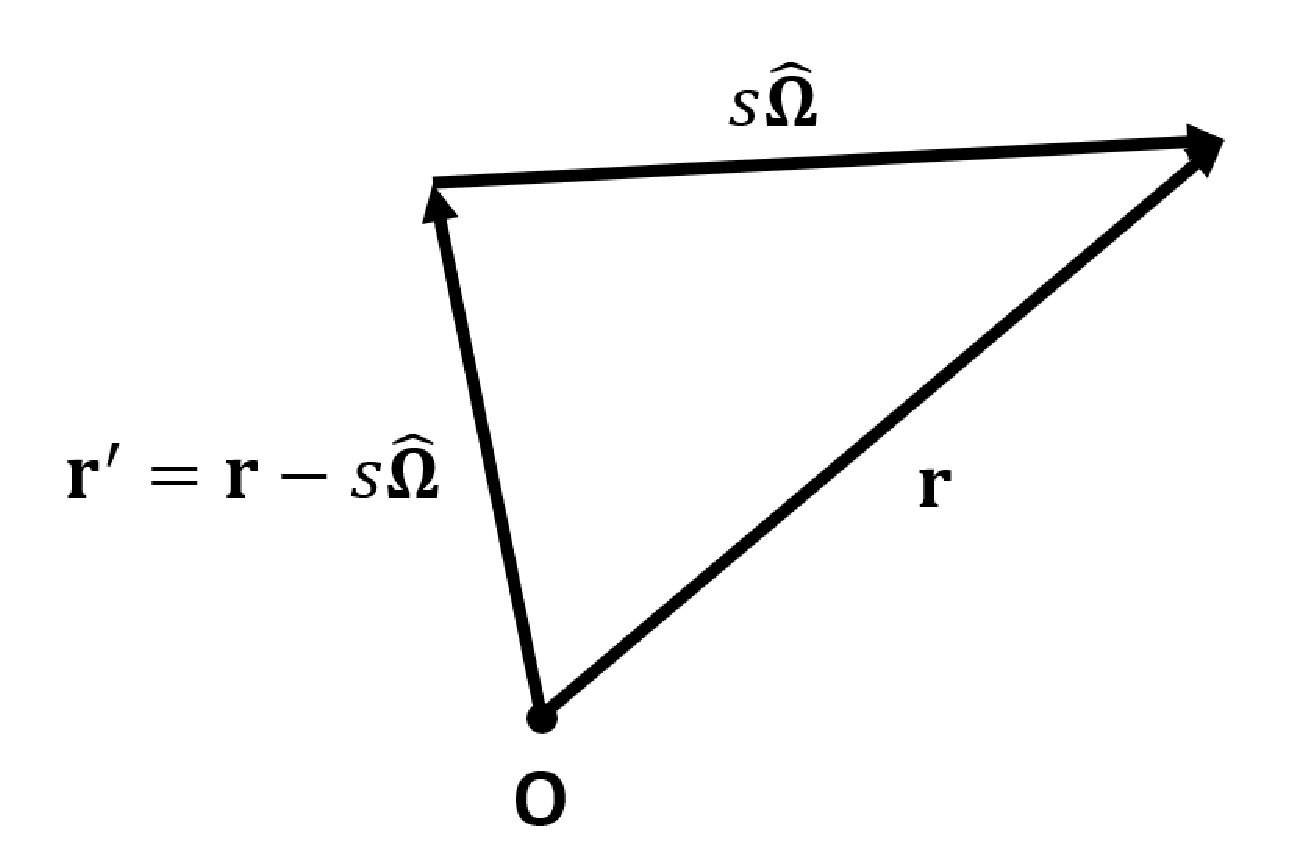
\includegraphics[width=80mm]{figure/path-s.eps}
  \caption{座標$\mathbf{r}'$の図示}\label{path-s}
  \end{center}
\end{figure}
\begin{equation}
  \mathbf{r}' = \mathbf{r} - s\SpcAng, \quad t' = t - \frac{s}{v}
\end{equation}
である。あるスカラーの関数$f(\mathbf{r}', t')$について、
$\mathbf{r}'(s), t'(s)$の合成関数と見れば、今表現したい微分は
\begin{align}
  \frac{df}{ds}
  \ = \frac{\partial f}{\partial \mathbf{r}'} \frac{\partial \mathbf{r}'}{\partial s} + \frac{\partial f}{\partial t'} \frac{\partial t'}{\partial s}
  \ = \frac{\partial f}{\partial \mathbf{r}'} \cdot (-\SpcAng) + \frac{\partial f}{\partial t'} (-\frac{1}{v})
  \ = -\SpcAng \cdot \nabla' f - \frac{1}{v} \frac{\partial f}{\partial t'}
\end{align}
角度中性子束$\psi$についてこの微分を考えれば、中性子が飛行している方向に沿って移動しながら、
角度束がどう変わっていくかを示す微分となる。そして、中性子輸送方程式の
漏洩率と時間変化部分はこの微分で置き換えられることが分かる。
よって、座標を$(\mathbf{r}', t')$に置き換えた中性子輸送方程式~\eqref{trans-Q}は
\begin{equation}
  \left( \frac{d}{ds} - \Sigma_t(\mathbf{r} - s\SpcAng, E) \right) \psi(\mathbf{r} - s\SpcAng, E, \SpcAng, t - s/v) = 
  -Q(\mathbf{r} - s\SpcAng, E, \SpcAng, t - s/v) \label{trans-s}
\end{equation}
となる。この微分方程式は

\begin{equation}
  \frac{df(s)}{ds} + P(s)f(s) = Q(s)
\end{equation}

の形をしている非斉次一階線形微分方程式で、積分因子法を用いて解くことができる。
積分因子法は

\begin{equation}
  g(s) \left( \frac{df(s)}{ds} + P(s)f(s) \right) = \frac{d}{ds} \left( g(s) f(s) \right) \label{Int-factor}
\end{equation}

となるように積分因子$g(s)$を決めれば、
\begin{equation}
  \frac{d}{ds} \left( g(s) f(s) \right) = g(s) Q(s)
\end{equation}
となり、積分により$g(s)f(s)$が求まるという解法である。
積分因子の条件~\eqref{Int-factor}より、

\begin{align}
  &\text{左辺は} \quad g(s) \left( \frac{df}{ds} + P(s) f \right) = g(s) \frac{df}{ds} + g(s) P(s) f \notag\\
  &\text{右辺は} \quad \frac{d}{ds} \left( g(s) f(s) \right) = g(s) \frac{df}{ds} + \frac{dg}{ds} f \notag \\
\end{align}

両辺を見比べると$g(s) \frac{df}{ds}$が削除出来て、積分因子は

\begin{equation}
  \frac{dg}{ds} = g(s) P(s)
\end{equation}

を満たさなければならない。
したがって、式~\eqref{trans-s}の積分因子は
\begin{align}
  \frac{dg}{ds} &= -\Sigma_t(\mathbf{r} - s\SpcAng, E) g(s) \notag \\
  \frac{dg}{g} &= -\Sigma_t(\mathbf{r} - s\SpcAng, E) \ ds \notag \\
  \int_{0}^{s} \frac{1}{g} \frac{dg}{ds} \ ds &= \int_{0}^{s} -\Sigma_t(\mathbf{r} - s\SpcAng, E,E) \ ds' \notag \\
  \ln{g(s)} - \ln{g(0)} &= - \int_{0}^{s} \Sigma_t(\mathbf{r} - s'\SpcAng, E) \ ds' \notag \\
  \text{$g(0)=1$として} \quad g(s) &= \mathrm{exp} \left( - \int_{0}^{s} \Sigma_t(\mathbf{r} - s'\SpcAng, E) \ ds' \right) \label{trans-Int-factor}
\end{align}
この積分因子を式~\eqref{trans-s}の両辺に掛けると

%\newcommand{\gs}{\mathrm{exp} \left( - \int_{0}^{s} \Sigma_t(\mathbf{r} - s'\SpcAng) \ ds' \right)}
%\newcommand{\gsd}{\mathrm{exp} \left( - \int_{0}^{s'} \Sigma_t(\mathbf{r} - s''\SpcAng) \ ds'' \right)}
\newcommand{\gs}{e^{ - \int_{0}^{s} \Sigma_t(\mathbf{r} - s'\SpcAng) \ ds' }}
\newcommand{\gsd}{e^{ - \int_{0}^{s'} \Sigma_t(\mathbf{r} - s''\SpcAng) \ ds'' }}
\newcommand{\rsO}{\mathbf{r} - s\SpcAng}
\newcommand{\rsdO}{\mathbf{r} - s'\SpcAng}
\newcommand{\tsv}{t - s/v}
\newcommand{\tsdv}{t - s'/v}
\begin{align}
  \frac{d}{ds} \left[ \gs \psi(\rsO, \tsv) \right] \notag\\
   = - \gs Q(\rsO, \tsv)
\end{align}
なお、表記の簡略化のためエネルギーと飛行方向の変数$E, \SpcAng$を省いた。
この式を$0 \rightarrow s$で積分すれば、角度束$\psi$についての式を得ることが出来る。
左辺について、
\begin{align}
  &\int_0^s \frac{d}{ds'} \left[ \gsd \psi(\rsdO, \tsdv) \right] \ ds' \notag \\
  &= \left[ \gsd \psi(\rsdO, \tsdv) \right]_0^s \notag \\
  &= \gs \psi(\rsO, \tsv) - \mathrm{exp}(0) \psi(\mathbf{r}, t)
\end{align}
なので、輸送方程式は
\begin{align}
  \psi(\rEOt) = e^{-\int_{0}^{s} \Sigma_t(\mathbf{r} - s'\SpcAng, E) \ ds'} \psi(\rsO, E, \SpcAng, \tsv) \notag \\
  + \int_0^s \left[ e^{-\int_{0}^{s'} \Sigma_t(\mathbf{r} - s''\SpcAng, E) \ ds''} Q(\rsdO, E, \SpcAng, \tsdv) \right] \ ds' \label{int-trans-pre}
\end{align}
となる。

この式の物理的意味は次のように説明できる。
右辺第1項は$s$だけ巻き戻された$\SpcAng$方向の角度束に、位置$\mathbf{r}$まで衝突せずに
進む確率$\gs$を掛けたものである。右辺第2項の被積分関数は、線源または散乱によって生成される
$s'$だけ巻き戻された位置、時刻の中性子数に$s'$の距離を衝突せずに進む確率$\gsd$を掛けたもの
である。これを$0$から$s$まで積分したものが右辺第2項となる。

この式を導出する際の積分範囲を$s \rightarrow \infty$とすると右辺第1項が消えて、
積分型中性子輸送方程式となる。
\vskip.5\baselineskip
\begin{itembox}[l]{積分型中性子輸送方程式}
  \begin{equation}
    \psi(\rEOt) 
    = \int_{0}^{\infty} e^{ - \int_{0}^{s} \Sigma_t(\mathbf{r} - s'\SpcAng, E) \ ds'} Q(\rsO, E, \SpcAng, \tsv) \ ds \label{int-trans}
  \end{equation}
  ただし、$Q(\rsO, E, \SpcAng, \tsv)$は
  \begin{align}
    &Q(\rsO, E, \SpcAng, \tsv) = \notag \\
    &\int_{4 \pi} \int_{0}^{\infty} \left[  
    \Sigma_s (\rsO, \EOtoEO) \psi(\rsO, E', \SpcAng', \tsv) \right] dE' d\SpcAng' \notag\\
    &+ s(\rsO, E, \SpcAng, \tsv)
  \end{align}
\end{itembox}
\vskip.5\baselineskip
これは微積分型輸送方程式~\eqref{transport}に、無限遠で角度束が$0$となる境界条件を
あたえたものと等価である。
式~\eqref{int-trans-pre}と~\eqref{int-trans}は共に格子体系の中性子束計算によく使われる。

\newpage